{\color{Blue}{\subsection{Implementation}}}
{\setlength{\parskip}{0.5cm}
It has been decided that, as there is the presence of two partly distinguished applications, the implementation will be led concurrently by two different teams. In this way it will be possible to not lose time during the integration and testing part. Each team will focus on one client application, performing firstly implementation and then unit testing of each coded module. 


{\color{Blue}{\subsubsection{Client Applications}}}
Both the teams will work in a joint session to develop the part related to the sensor interaction. The first task will be the implementation of the DeviceProxy module that will interface with the real devices through the available APIs. The second will be the realization of the DeviceManager and consequent test. Then a week will be taken to discuss and choose the most efficient algorithms for collecting data, that could be handled by the DataCollector, implemented as third. It will be important to provide some simple test cases to perform unit testing of this component owing to its complexity in handling sensor data. After that, the two teams will work separately for the remaining components of the client application.

{\color{Blue}{\subsubsection{Server Application}}}
Once finished the implementation of the smartphone apps, both the teams will manage the server architecture. Firstly, they will concentrate their efforts on the most complex module: the Analyzer. In collaboration with biomedical engineers and medical researchers, this component will be firstly defined in detail, then implemented. The whole process is expected to be completed in at least one month, a couple of weeks will be taken to create test cases and perform unit testing of the mentioned module.\\
Completed this phase, the two teams will separate to code and test the following units:
\begin{itemize}
	\item {First Team, Session Management:
	\begin{itemize}
		\item \textbf{SessionManager}
		\item \textbf{Session, UserDataQueue, UserDataStream}
		\item \textbf{Dispatcher}
	\end{itemize}}
	\item {Second Team, Emergency Management
	\begin{itemize}
		\item \textbf{EmergencyCondition, AnomalyCondition}
		\item \textbf{ERMManager}
		\item \textbf{Resource}
	\end{itemize}}
\end{itemize}
Then both the teams will work jointly on:
\begin{itemize}[topsep=-0.2em]
	\item \textbf{HealthProfileManager}
	\item \textbf{SupervisorManager}
	\item \textbf{DatabaseManager:} in particular, the part concerning ASOS functionalities;
	\item \textbf{EventObserver} and \textbf{EventHandling Interface}: at least to allow message exchanging for what concerns ASOS client-server communication.
\end{itemize}
After this working session the integration and testing phases could start for the implemented architecture, carried on by one of the two teams. The decision to following this order has been taken since it is almost intuitive that the mentioned phases will take much more time than the ones required for the rest of the architecture.
%In order to better understand the following explanation, please refer to Fig.~\ref{figura3}.\\
%The Data4Help client part presents only one criticality, that is the Hardware Interaction. Is essential that the data provided by the devices are managed correctly by the application and then sent. Hence this is the part that has to be implemented first as common to both the applications. The implementation of the first part of the first team will follow this order:
Meanwhile, the other team will focus on the part of the server architecture that regards D4H functionalities, coding the remaining part of the DatabaseManager.

%{\color{Blue}{\subsubsection{AutomatedSOS}}}

%In order to better understand the following explanation, please refer to Fig.~\ref{figura3}.\\
%As for the Data4Help client part, and even more since we have to deal with people's life, the critical part is the Hardware Interaction. This part will be developed first, followed by the others.
%The second team will work in server architecture implementation, starting with  In the while if the first team successfully finished the app implementation and unit testing, it wil join with the second team in implementing server components regarding D4H functionalities.

%{\color{Blue}{\subsubsection{Common part}}}
%In order to better understand the following explanation, please refer to Fig.~\ref{figura4}.\\
%The component that is mandatory to be implemented first is the Analyzer. It is the core of AutomatesSOS system, the one that receives the data and decides if there is something wrong with them. Consequently the second part to be developed is the Emergency and Anomaly condition components. After a detection is important that the condition is managed in the correct way. Once completed these parts, the connection between the ERMManager and the Resource components and them must be done.
%After that, the Session, the SessionManager and the Dispatcher have to be implemented. In this way, the entire managing of a piece of data is completed, from the arriving to a possible problem detection.
%The remaining parts can be now developed. 


{\color{Blue}{\subsection{Integration and Testing}}}
The integration and testing part will be performed bottom-up. This decision has been taken because these two applications have more critical parts in the business logic components and client-server communications, instead of the user/application interactions. The bottom-up model permits us to start by creating a solid base, starting to test the client architecture, then the server one and finally the communication between the two parts.

{\color{Blue}{\subsubsection{Client: Data4Help and AutomatedSOS Testing}}}
The integration part will be done following the implementation part. This means that as soon as a component will be ready, the integration with the other ones already available will be performed.\\
The first test will be carried out on the sensor interaction part, involving the DeviceProxy, DataCollector and DeviceManager. Different test cases will feed the integrated modules in order to evaluate their response under stressing workloads and that of external devices when communicating with the DeviceProxy. \\
After the unit testing of the other client components and their integration with the EventObserver through the EventHandling interface, the client architecture can be tested feeding both the apps with patterns of messages to test the client reaction to external events. Few days could be required to decide which test cases are the most suitable for this testing phase.
%Testing will be performed using data concerning different types of physical control (like Heart Rate, Blood Pressure of body temperature) and trying to send as many data as possible in order to stress the system. Testing will be considered successfully completed if the application will be able to process and send correctly those data. 

{\color{Blue}{\subsubsection{Server-side Testing}}}
The server logic is the hardest part for testing phase. As said in the previous section, as soon as the Analyzer unit is coded and tested, it must be integrated with the EmergencyCondition and AnomalyCondition components once they had been completed. In the while, if the first team coded the Resource and ERMManager components, a Driver and a Stub components could be created to simulate the EmergencyCondition block (based on the current work of the other team) and the behavior of the real ERM. All of this, to test the ERM communication part:
\begin{figure}[H]
	\centering
	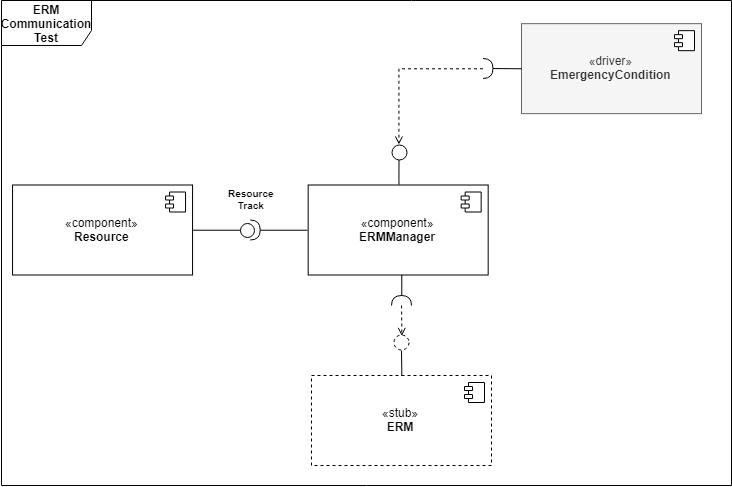
\includegraphics[scale=0.4]{Images/uml/erm_testing.png}
	\label{figure19}
	\caption{ERM Communication Testing}
\end{figure}

After this moment, for a couple of weeks, several test cases will be discussed and inserted in the test plan in order to optimize the resources spent during this phase. Once the previous tasks are completed the developed part of architecture will be tested using the chosen cases, after the relative stub and driver components are created:

\begin{figure}[H]
	\centering
	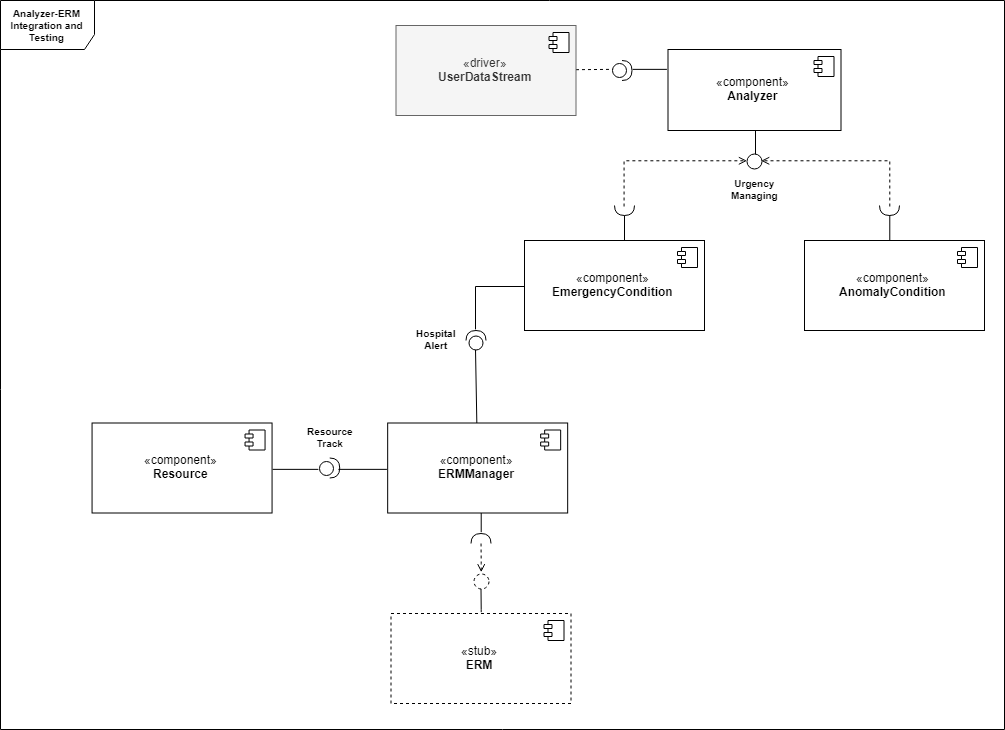
\includegraphics[scale=0.4]{Images/uml/analyzer_integrationtesting.png}
	\label{figure20}
	\caption{Analyzer-ERM Integration and Testing}
\end{figure}

After this long test step, the developed architecture will be integrated with the Session Management part and the other components, once these ones are completed and tested as well.\\
For what concerns D4H part of the architecture at server side, a particular attention should be spent to the interaction between the third parties and the user datasets and in particular to the PrivacyAndSecurityEvaluator. At this point, for few days, several test cases will be inserted in this part of the test plan with the support of computer security engineers. Once the TP\_RequestManager, the mentioned security module and the DatasetGenerator are completed, the integration and consequent test of these components can be performed.\\
After that the DatabaseManager and EventObserver can be integrated to the rest of the architecture and lastly tested.\\
At the end of this long phase, the two teams are expected to work together on a set of test cases to stress the entire system and in particular the communication between client and server applications. This last phase is clearly explained in the next section.

{\color{Blue}{\subsubsection{Communication Testing}}}
%As already said in the previous subchapter, also for this part, the integration will follow the steps of the implementation.
%For what concerns the testing part, it will start by giving to the Analyzer fake types of data in order to verify that it could interpret them in the correct way and discover emergency or anomaly conditions. As soon as the other parts will be ready they will be add and it will be verified the operating giving fake emergency or anomalies condition type of data.
The last part of testing will be performed once every part of the two architectures will be completed. It consists on trying to make client and server working together preventing any conflict between them. Here is a list of special test cases required to probe the communication and reaction of the system when conflict events occur:
\begin{itemize}
\item\textbf{Register a device when AsosMonitorMode is activated:} in order to not create any conflict, the system must prevent the user to add a new device while ASOS is working.% In this way is possible to test the communication between the SessionManager and the EventObserver at both sides, in synchronizing the activities.
In this case a warning should be showed to the user. 
\item\textbf{Turn on AsosMonitorMode while Data4Help is collecting data:} the system should let the user to start an ASOS session. The result should consist on stopping the collection of data from a specific device in Data4Help, in order to not create sample copies collected by both the running applications, if one or more devices working with D4H are required by ASOS. At server side the expected result is a change in the state of the Session and the Dispatcher that will push the new set of samples into the UserDataStream  while continuing to fulfill the relative queue. The mentioned set will be committed anyway to the database.
\item\textbf{Turn off AsosMonitorMode while Data4Help is collecting data:} the system should return in the state it was before turning on the AsosMonitorMode. Samples should not be sent to the UserDataStream anymore.
\end{itemize}
}










